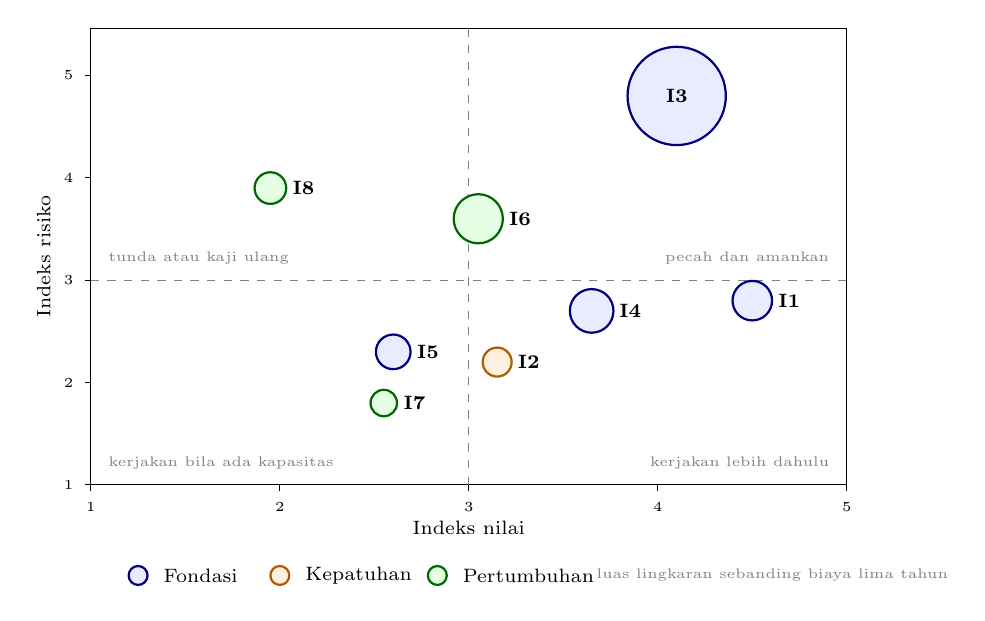
\begin{tikzpicture}[
  font=\scriptsize,
  fondasi/.style={draw=blue!50!black, fill=blue!8, thick},
  kepatuhan/.style={draw=orange!70!black, fill=orange!12, thick},
  tumbuh/.style={draw=green!40!black, fill=green!10, thick},
  kode/.style={font=\scriptsize\bfseries, anchor=west, inner sep=1pt}
]
  % Sumbu: indeks nilai 1 sampai 5 menjadi 0 sampai 9,6 cm,
  % indeks risiko 1 sampai 5 menjadi 0 sampai 5,2 cm.
  \draw (0,0) rectangle (9.6,5.8);
  \draw[gray, dashed] (4.8,0) -- (4.8,5.8);
  \draw[gray, dashed] (0,2.6) -- (9.6,2.6);
  \foreach \nilai/\posisi in {1/0, 2/2.4, 3/4.8, 4/7.2, 5/9.6} {
    \draw (\posisi,0) -- (\posisi,-0.08);
    \node[anchor=north, font=\tiny] at (\posisi,-0.1) {\nilai};
  }
  \foreach \risiko/\posisi in {1/0, 2/1.3, 3/2.6, 4/3.9, 5/5.2} {
    \draw (0,\posisi) -- (-0.08,\posisi);
    \node[anchor=east, font=\tiny] at (-0.1,\posisi) {\risiko};
  }
  \node at (4.8,-0.55) {Indeks nilai};
  \node[rotate=90] at (-0.6,2.9) {Indeks risiko};

  \node[font=\tiny, gray, anchor=south east] at (9.5,0.08) {kerjakan lebih dahulu};
  \node[font=\tiny, gray, anchor=south east] at (9.5,2.68) {pecah dan amankan};
  \node[font=\tiny, gray, anchor=south west] at (0.1,2.68) {tunda atau kaji ulang};
  \node[font=\tiny, gray, anchor=south west] at (0.1,0.08) {kerjakan bila ada kapasitas};

  % Jari-jari 0,09 kali akar biaya, sehingga luas lingkaran sebanding biaya.
  \draw[fondasi] (7.44,4.94) circle (0.624);
  \node[font=\scriptsize\bfseries] at (7.44,4.94) {I3};
  \draw[fondasi] (8.40,2.34) circle (0.251);
  \node[kode] at (8.69,2.34) {I1};
  \draw[fondasi] (6.36,2.21) circle (0.277);
  \node[kode] at (6.67,2.21) {I4};
  \draw[fondasi] (3.84,1.69) circle (0.220);
  \node[kode] at (4.10,1.69) {I5};
  \draw[kepatuhan] (5.16,1.56) circle (0.184);
  \node[kode] at (5.38,1.56) {I2};
  \draw[tumbuh] (4.92,3.38) circle (0.312);
  \node[kode] at (5.27,3.38) {I6};
  \draw[tumbuh] (3.72,1.04) circle (0.168);
  \node[kode] at (3.93,1.04) {I7};
  \draw[tumbuh] (2.28,3.77) circle (0.201);
  \node[kode] at (2.52,3.77) {I8};

  \draw[fondasi] (0.6,-1.15) circle (0.12);
  \node[anchor=west] at (0.8,-1.15) {Fondasi};
  \draw[kepatuhan] (2.4,-1.15) circle (0.12);
  \node[anchor=west] at (2.6,-1.15) {Kepatuhan};
  \draw[tumbuh] (4.4,-1.15) circle (0.12);
  \node[anchor=west] at (4.6,-1.15) {Pertumbuhan};
  \node[anchor=west, font=\tiny, gray] at (6.3,-1.15)
    {luas lingkaran sebanding biaya lima tahun};
\end{tikzpicture}
